\documentclass[11pt]{article}

\usepackage{amsmath,amssymb}
\usepackage{hyperref}
\usepackage{enumitem}
\usepackage{geometry,comment}
\usepackage{xcolor}
\geometry{margin=1in}
\usepackage{tikz}
\usetikzlibrary{decorations.pathreplacing}
\usepackage{tikz-cd}
\usepackage{pgfplots}
\usepackage[binary-units=true]{siunitx}
\usepackage{graphicx}
\usepackage[font=small]{caption}
\usepackage[most]{tcolorbox}

\title{SP1 zkVM Architecture}
\author{Succinct Labs\\[8pt]}

\newcommand{\bwnote}[1]{%
    {\color{red}\textbf{Benedikt says:} #1}%
}

\newcommand{\dknote}[1]{%
    {\color{magenta}\textbf{Dmitry says:} #1}%
}

\newtcolorbox{instruction}{%
  colback=teal!8,%
  colframe=teal!50!black,%
  fontupper=\sffamily\small\color{teal!40!black},%
  boxrule=0.5pt,%
  arc=2pt,%
  left=6pt,right=6pt,top=4pt,bottom=4pt%
}
\newcommand{\aznote}[1]{%
	{\color{blue}\textbf{Arantxa:} #1}%
}
\newcommand{\gknote}[1]{%
	{\color{purple}\textbf{George:} #1}%
}
\newcommand{\PPP}{\mathcal{P}} %Program
\newcommand{\III}{\mathcal{I}} %Input
\newcommand{\OOO}{\mathcal{O}} %Output
\newcommand{\WWW}{\mathcal{W}} %Witness
\newcommand{\BBB}{\mathcal{B}} %Basic block

\newcommand{\predicate}{\mathbf{P}}

\newcommand{\TTT}{\mathcal{T}} %Trace
\newcommand{\EE}{\mathbb{E}} %Ethereum state
\newcommand{\GGG}{\mathcal{G}} %Segment

\newcommand{\code}{\mathtt{code}} %Code of a segment
\newcommand{\state}{\mathcal{S}} %State of a segment
\newcommand{\mem}{\mathtt{mem}}
\newcommand{\regs}{\mathtt{regs}}
\newcommand{\pc}{\mathtt{pc}}
\newcommand{\seg}{\mathrm{seg}}
\newcommand{\www}{\mathsf{w}} %Witness for a step

\newcommand{\relation}{\mathcal{R}}

\newcommand{\Com}{\mathrm{Com}} %Commitment to memory
\newcommand{\pred}[1]{\ensuremath{\varphi_{\mathrm{#1}}}} %Predicate for operations
\newcommand{\op}{\mathrm{op}} %Operation code
\newcommand{\rea}{\mathrm{read}} %Read operation code
\newcommand{\writ}{\mathrm{write}} %Write operation code
\newcommand{\step}{\mathrm{step}} %Relation for segment trace (inner-step)
\newcommand{\keccak}{\mathrm{keccak}} %Relation for keccak precompile
\newcommand{\poseidon}{\mathrm{poseidon}} %Relation for poseidon precompile
\newcommand{\range}{\mathrm{range}} %Relation for range checks
\newcommand{\bus}{\mathrm{bus}} %Relation for bus steps
\newcommand{\Vfy}{\mathsf{V}} %Shorthand for Verify

\newtheorem{claim}{Claim}
\date{\today}
\begin{document}

\maketitle

\section*{Overview}

This document describes the architecture of the \textbf{SP1 zkVM}
according to the W1 deliverable of the EF zkVM whitepaper
guidelines\footnote{\url{https://zkevm.ethereum.foundation/blog/cryptography-research-update}}.
SP1 proves execution of RISC-V guest programs using:

\begin{itemize}
\item Execution of RV64IM programs compiled from ELF binaries
\item Sharded execution traces with chip-cluster--based segmentation
\item Specialized constraint systems (``chips'') grouped into clusters
\item Local bus interactions (LogUp + GKR) within each shard
\item Global bus interactions across shards (septic curve accumulation)
\item Hypercube proof system with BaseFold polynomial commitments over the KoalaBear field
\item Recursive aggregation via normalize / compose / shrink circuits
\end{itemize}

After execution, the trace is partitioned into \emph{shards}, each corresponding to a chip cluster instance.
Every shard is proven independently, producing a core shard proof.
These proofs are then normalized to a fixed shape and recursively aggregated until a single proof attests to the correctness of the entire program execution.

\section{Execution Model}
We define how a program is executed.

\subsection{Program, Execution, and VM State}

A \textbf{program} $\PPP$ is a RISC-V ELF binary targeting the RV64IM
instruction set (64-bit base integer with multiply/divide extension).
Its inputs $\III$ are derived from the Ethereum state (\emph{initial state})
and the execution witness $\WWW$,
and its outputs $\OOO$ are the final Ethereum state (\emph{final state}).

The program $\PPP$ operates on the \textbf{VM state} $S$, defined as:
\begin{itemize}
\item $\pc$: 64-bit program counter
\item $\regs[0..31]$: 32 general-purpose registers (x0--x31), each 64 bits wide,
      with x0 hardwired to zero
\item $\mem[]$: byte-addressed writable memory
\end{itemize}
We separately denote the code of the program by $\code$. It is immutable and read-only, and is not part of the VM state.

A single instruction step of the program execution is defined as a transition from
one VM state to another according to the semantics of the instruction $\op$ retrieved from
$\code$ at the program counter $\pc_1$. This is denoted as follows:
\begin{equation}\label{eq:op}
S:=(\pc_1,\regs_1,\mem_1)\xrightarrow{\op:=\code[\pc_1]} S':=(\pc_2,\regs_2,\mem_2)
\end{equation}
For example, if $\op$ is an addition instruction, which adds the first two registers and stores in the third register, then the semantics of the step is defined as
\begin{align}
\pc_2&=\pc_1+1,\\
\regs_2&=\regs_1\text{ except that } \regs_2[2]:=\regs_1[0]+\regs_1[1],\\
\mem_2&=\mem_1.
\end{align}
We will use the notation $(\pc_1,\regs_1,\mem_1)\rightarrow  (\pc_2,\regs_2,\mem_2)$ to denote that $S$ transitions to $S'$ by executing instruction
 $\op:=\code[\pc_1]$.


An \textbf{execution trace} for program $\code$ applied to inputs $\III$ is a sequence of VM states

\[
\TTT:\quad S_0 \rightarrow S_1 \rightarrow \cdots \rightarrow S_T
\]
where each step corresponds to execution of one instruction.


A \textbf{zkVM proof} for $(\PPP,\EE,\EE')$,
where $\EE$ and $\EE'$ are the initial and final Ethereum states, is a SNARK that proves the following:
$$
\begin{cases}
S_0\rightarrow\cdots\rightarrow S_T;\\
S_0:=(\pc_0:=0,\regs,\mem)\text{ where $\regs,\mem$ are derived from }\EE;\\
S_T:=(\pc_T,\regs',\mem')\text{ where $\regs',\mem'$ are derived from }\EE';\\
\end{cases}
$$

\subsection{Supported Instructions}
SP1 supports the full RV64IM instruction
set\footnote{\url{https://riscv.org/technical/specifications/}}:
the base 64-bit integer instructions (I) and the integer
multiply/divide extension (M).
Additionally, SP1 provides \emph{precompiles}---accelerated
implementations of expensive operations---invoked via the RISC-V
\texttt{ecall} instruction with a syscall code in register \texttt{t0}.

The precompiles include:
\begin{itemize}
\item \textbf{Hash functions:} SHA-256 (extend + compress), Keccak-256
  permutation, Poseidon2.
\item \textbf{Elliptic curve operations:} point addition, doubling, and
  decompression for Ed25519, Secp256k1, Secp256r1, BN-254, and
  BLS12-381.
\item \textbf{Field arithmetic:} $\mathbb{F}_p$ and $\mathbb{F}_{p^2}$
  add/sub/mul for BN-254 and BLS12-381.
\item \textbf{Big-integer arithmetic:} 256-bit multiply, 256-bit
  add/multiply with carry, $256\times 2048$-bit multiply.
\item \textbf{System:} halt, I/O (write, hint read/len), commit,
  deferred proof verification, memory protection.
\end{itemize}

For our purpose the exact semantics of each instruction is not
important; we treat them as black boxes with predicates modeling
correctness.
For a given instruction $\op$, the predicate $\varphi_{\op}$ has the
semantics
\begin{multline}\label{eq:phiop}
\varphi_{op}(\pc_1,\regs_1,\mem_1,\pc_2,\regs_2,\mem_2)=\mathrm{TRUE} \;\Longleftrightarrow\;\\
 (\pc_1,\regs_1,\mem_1)\xrightarrow{\op} (\pc_2,\regs_2,\mem_2) \wedge \code[\pc_1]=op
\end{multline}


\section{Segmentation}
We now explain how execution is split into shards.

\subsection{Execution Shards}

\begin{figure}
\centering
\resizebox{\textwidth}{!}{%
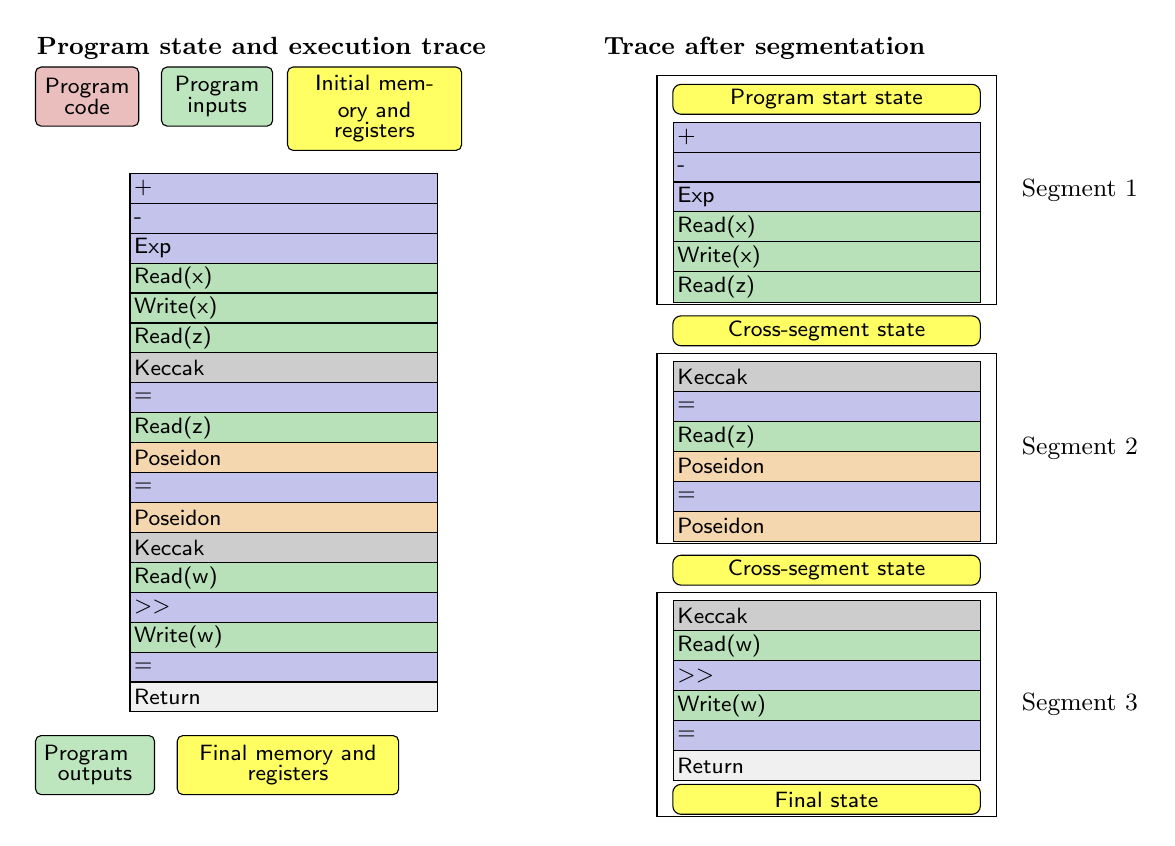
\begin{tikzpicture}[y=-1cm]
  % Colors
  \definecolor{alucol}{RGB}{195,195,235}
  \definecolor{memcol}{RGB}{185,225,185}
  \definecolor{hashcol}{RGB}{205,205,205}
  \definecolor{poscol}{RGB}{245,215,175}
  \definecolor{retcol}{RGB}{240,240,240}
  \definecolor{codecol}{RGB}{235,190,190}
  \definecolor{inputcol}{RGB}{190,230,190}
  \definecolor{statecol}{RGB}{255,255,100}
  %
  \def\rh{0.38}
  \def\bw{3.8cm}
  %
  \tikzset{
    ibox/.style={draw, thin, minimum height=\rh cm, text width=\bw, inner sep=1.5pt,
                 anchor=north west, font=\footnotesize\sffamily},
    sbox/.style={draw, thin, rounded corners=3pt, fill=statecol, minimum height=0.38cm,
                 text width=\bw, align=center, inner sep=1.5pt, font=\footnotesize\sffamily,
                 anchor=north},
    tbox/.style={draw, thin, rounded corners=2pt, minimum height=0.75cm, inner sep=3pt,
                 font=\footnotesize\sffamily, align=center, anchor=north west},
    seglabel/.style={font=\small, anchor=west},
  }
  %
  %%% LEFT SIDE %%%
  \node[anchor=north west, font=\small\bfseries] at (0, 0) {Program state and execution trace};
  %
  % Top boxes
  \node[tbox, fill=codecol, text width=1.1cm] at (0.1, 0.5) {Program\\[-2pt]code};
  \node[tbox, fill=inputcol, text width=1.2cm] at (1.7, 0.5) {Program\\[-2pt]inputs};
  \node[tbox, fill=statecol, text width=2.0cm] at (3.3, 0.5) {Initial memory and\\[-2pt]registers};
  %
  % Left instruction list (18 rows)
  \def\ly{1.85}
  \def\lx{1.3}
  \foreach \n/\txt/\col in {
    0/{+}/alucol, 1/{-}/alucol, 2/{Exp}/alucol,
    3/{Read(x)}/memcol, 4/{Write(x)}/memcol, 5/{Read(z)}/memcol,
    6/{Keccak}/hashcol, 7/{=}/alucol, 8/{Read(z)}/memcol,
    9/{Poseidon}/poscol, 10/{=}/alucol, 11/{Poseidon}/poscol,
    12/{Keccak}/hashcol, 13/{Read(w)}/memcol,
    14/{\textgreater\textgreater}/alucol, 15/{Write(w)}/memcol,
    16/{=}/alucol, 17/{Return}/retcol%
  } {
    \node[ibox, fill=\col] at (\lx, {\ly+\n*\rh}) {\txt};
  }
  %
  % Bottom boxes
  \node[tbox, fill=inputcol, text width=1.3cm] at (0.1, {\ly+18*\rh+0.3}) {\raggedright Program\\[-2pt]outputs};
  \node[tbox, fill=statecol, text width=2.6cm] at (1.9, {\ly+18*\rh+0.3}) {Final memory and\\[-2pt]registers};
  %
  %%% RIGHT SIDE %%%
  \def\rx{8.2}
  \pgfmathsetmacro{\rcx}{\rx + 1.953}
  %
  \node[anchor=north west, font=\small\bfseries] at (7.2, 0) {Trace after segmentation};
  %
  % --- Segment 1 ---
  \def\startY{0.72}
  \node[sbox] at (\rcx, \startY) {Program start state};
  %
  \pgfmathsetmacro{\segAy}{\startY + 0.48}
  \foreach \n/\txt/\col in {
    0/{+}/alucol, 1/{-}/alucol, 2/{Exp}/alucol,
    3/{Read(x)}/memcol, 4/{Write(x)}/memcol, 5/{Read(z)}/memcol%
  } {
    \node[ibox, fill=\col] at (\rx, {\segAy+\n*\rh}) {\txt};
  }
  %
  \pgfmathsetmacro{\segAtop}{\startY - 0.1}
  \pgfmathsetmacro{\segAbot}{\segAy + 6*\rh + 0.04}
  \draw[thin] ({\rx-0.2}, \segAtop) rectangle ({\rx+3.8+0.11+0.2}, \segAbot);
  \node[seglabel] at ({\rx+3.8+0.11+0.4}, {(\segAtop+\segAbot)/2}) {Segment 1};
  %
  % --- Cross-segment state 1 ---
  \pgfmathsetmacro{\isAy}{\segAbot + 0.14}
  \node[sbox] at (\rcx, \isAy) {Cross-segment state};
  %
  % --- Segment 2 ---
  \pgfmathsetmacro{\segBy}{\isAy + 0.58}
  \foreach \n/\txt/\col in {
    0/{Keccak}/hashcol, 1/{=}/alucol, 2/{Read(z)}/memcol,
    3/{Poseidon}/poscol, 4/{=}/alucol, 5/{Poseidon}/poscol%
  } {
    \node[ibox, fill=\col] at (\rx, {\segBy+\n*\rh}) {\txt};
  }
  %
  \pgfmathsetmacro{\segBtop}{\segBy - 0.1}
  \pgfmathsetmacro{\segBbot}{\segBy + 6*\rh + 0.04}
  \draw[thin] ({\rx-0.2}, \segBtop) rectangle ({\rx+3.8+0.11+0.2}, \segBbot);
  \node[seglabel] at ({\rx+3.8+0.11+0.4}, {(\segBtop+\segBbot)/2}) {Segment 2};
  %
  % --- Cross-segment state 2 ---
  \pgfmathsetmacro{\isBy}{\segBbot + 0.14}
  \node[sbox] at (\rcx, \isBy) {Cross-segment state};
  %
  % --- Segment 3 ---
  \pgfmathsetmacro{\segCy}{\isBy + 0.58}
  \foreach \n/\txt/\col in {
    0/{Keccak}/hashcol, 1/{Read(w)}/memcol,
    2/{\textgreater\textgreater}/alucol, 3/{Write(w)}/memcol,
    4/{=}/alucol, 5/{Return}/retcol%
  } {
    \node[ibox, fill=\col] at (\rx, {\segCy+\n*\rh}) {\txt};
  }
  %
  \pgfmathsetmacro{\finalY}{\segCy + 6*\rh + 0.05}
  \node[sbox] at (\rcx, \finalY) {Final state};
  %
  \pgfmathsetmacro{\segCtop}{\segCy - 0.1}
  \pgfmathsetmacro{\segCbot}{\finalY + 0.42}
  \draw[thin] ({\rx-0.2}, \segCtop) rectangle ({\rx+3.8+0.11+0.2}, \segCbot);
  \node[seglabel] at ({\rx+3.8+0.11+0.4}, {(\segCtop+\segCbot)/2}) {Segment 3};
\end{tikzpicture}%
}
\caption{Segmentation of the execution trace into 3 segments }\label{img:trace-seg}
\end{figure}

After execution, the execution trace $\TTT$ is divided into
\emph{shards} $\GGG_1,\GGG_2,\ldots,\GGG_m$
(cf.\ Fig.~\ref{img:trace-seg}).
Shards are not fixed-size; instead, the executor splits the trace when
the estimated trace area of the current shard exceeds a
configurable threshold\footnote{The default element threshold is
$2^{28}+2^{27}$, and the maximum table height per shard is $2^{22}$.}.
Each shard $\GGG_i$ corresponds to a contiguous subsequence of the
execution trace, from $S_{\mathrm{start}_i}$ to $S_{\mathrm{end}_i}$,
and is proven by its own core shard proof.

Sharding reduces the proof of the entire execution to proving the
validity of each shard and consistency between them.
The global consistency argument (enforced during recursive aggregation)
asserts:
$$
S_{\mathrm{end}_i} = S_{\mathrm{start}_{i+1}}\text{ for all }i\in[m-1],\quad S_{\mathrm{start}_1}=S_0,\quad S_{\mathrm{end}_m}=S_T.
$$

\subsection{Shard layout}

Each shard is proven by a \emph{chip cluster}---a collection of
chips (specialized constraint systems) that are included together in a
single proof.
The cluster determines which chips are present and thus the circuit
shape.
Within a shard, each chip produces a table of field elements
with algebraic constraints on its columns.
The full list of chip cluster types and their contents is given in
Section~\ref{sec:core}.

At a high level, every shard includes:
\begin{itemize}
\item An \textbf{execution trace chip} containing the RISC-V
  instruction steps, register accesses, and control flow for the
  shard's portion of execution.
\item \textbf{Precompile chips} for any accelerated operations invoked
  during the shard (e.g., SHA-256, Keccak, elliptic curve operations).
  Depending on cost, a precompile may be included in the same cluster
  as the execution trace or deferred to its own shard
  (Section~\ref{sec:core}).
\item \textbf{Infrastructure chips} for lookups (byte, range),
  memory state, timestamp management, syscall dispatch, and the global
  bus accumulator.
\end{itemize}

Consistency between chips within a shard is enforced by a \emph{bus}:
a LogUp interaction argument (proved via GKR) that checks that all
``send'' and ``receive'' messages across chips balance within the shard.

\begin{figure}
\centering
\resizebox{0.65\textwidth}{!}{%
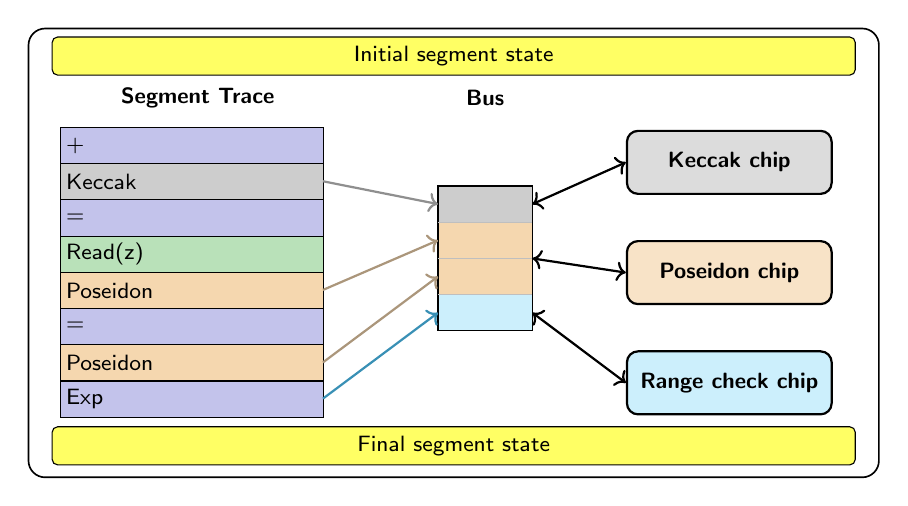
\begin{tikzpicture}[y=-1cm]
  % Colors
  \definecolor{alucol}{RGB}{195,195,235}
  \definecolor{memcol}{RGB}{185,225,185}
  \definecolor{hashcol}{RGB}{205,205,205}
  \definecolor{poscol}{RGB}{245,215,175}
  \definecolor{statecol}{RGB}{255,255,100}
  \definecolor{buscol}{RGB}{255,195,115}
  %
  \def\rh{0.46}
  %
  \tikzset{
    ibox/.style={draw, thin, minimum height=\rh cm, text width=3.2cm, inner sep=2pt,
                 anchor=north west, font=\footnotesize\sffamily},
    chip/.style={draw, thick, rounded corners=4pt, minimum width=2.6cm, minimum height=0.8cm,
                 font=\footnotesize\sffamily\bfseries, align=center},
    sbar/.style={draw, thin, rounded corners=2pt, fill=statecol,
                 minimum height=0.42cm, minimum width=10.2cm,
                 font=\footnotesize\sffamily},
  }
  %
  % Layout constants
  \def\tx{0.4}     % trace x
  \def\trw{3.34}   % trace box total width (3.2 text + 0.14 inner sep)
  \def\busx{5.2}   % bus x (shifted right for arrow space)
  \def\busw{1.2}   % bus width
  \def\ty{1.25}    % trace y start
  \def\bsy{2.0}    % bus start y (shorter than trace)
  %
  % === BIG ENCLOSING BOX ===
  \draw[semithick, rounded corners=6pt] (0, 0) rectangle (10.8, 5.7);
  %
  % === INITIAL STATE BAR ===
  \node[sbar] at (5.4, 0.35) {Initial segment state};
  %
  % === COLUMN LABELS ===
  \node[font=\footnotesize\sffamily\bfseries] at (2.15, 0.88) {Segment Trace};
  \node[font=\footnotesize\sffamily\bfseries] at ({\busx + \busw/2}, 0.88) {Bus};
  %
  % === INSTRUCTION ROWS (color-coded by chip affiliation) ===
  \foreach \n/\txt/\col in {
    0/{+}/alucol,
    1/{Keccak}/hashcol,
    2/{=}/alucol,
    3/{Read(z)}/memcol,
    4/{Poseidon}/poscol,
    5/{=}/alucol,
    6/{Poseidon}/poscol,
    7/{Exp}/alucol%
  } {
    \node[ibox, fill=\col] at (\tx, {\ty+\n*\rh}) {\txt};
  }
  %
  % === BUS COLUMN (only precompile/range-check entries, colored by chip) ===
  % 4 cells: Keccak, Poseidon, Poseidon, Range check
  \fill[hashcol]  (\busx, \bsy) rectangle ({\busx+\busw}, {\bsy+\rh});
  \fill[poscol]   (\busx, {\bsy+\rh}) rectangle ({\busx+\busw}, {\bsy+2*\rh});
  \fill[poscol]   (\busx, {\bsy+2*\rh}) rectangle ({\busx+\busw}, {\bsy+3*\rh});
  \fill[cyan!20]  (\busx, {\bsy+3*\rh}) rectangle ({\busx+\busw}, {\bsy+4*\rh});
  % Grid
  \draw[thin] (\busx, \bsy) rectangle ({\busx+\busw}, {\bsy+4*\rh});
  \foreach \n in {1,2,3} {
    \draw[thin, black!25] (\busx, {\bsy+\n*\rh}) -- ({\busx+\busw}, {\bsy+\n*\rh});
  }
  %
  % === ARROWS: TRACE → BUS ===
  \pgfmathsetmacro{\trR}{\tx + \trw}  % trace right edge
  % Keccak (trace row 1) → bus cell 0
  \draw[->, thick, hashcol!70!black] (\trR, {\ty+1*\rh+\rh/2}) -- (\busx, {\bsy+\rh/2});
  % Poseidon (trace row 4) → bus cell 1
  \draw[->, thick, poscol!70!black] (\trR, {\ty+4*\rh+\rh/2}) -- (\busx, {\bsy+\rh+\rh/2});
  % Poseidon (trace row 6) → bus cell 2
  \draw[->, thick, poscol!70!black] (\trR, {\ty+6*\rh+\rh/2}) -- (\busx, {\bsy+2*\rh+\rh/2});
  % Exp/range check (trace row 7) → bus cell 3
  \draw[->, thick, cyan!70!black] (\trR, {\ty+7*\rh+\rh/2}) -- (\busx, {\bsy+3*\rh+\rh/2});
  %
  % === FINAL STATE BAR ===
  \node[sbar] at (5.4, 5.3) {Final segment state};
  %
  % === CHIP BOXES (spread across full trace height) ===
  \node[chip, fill=hashcol!70] (sha3chip) at (8.9, 1.7) {Keccak chip};
  \node[chip, fill=poscol!70] (poschip) at (8.9, 3.1) {Poseidon chip};
  \node[chip, fill=cyan!20] (rangechip) at (8.9, 4.5) {Range check chip};
  %
  % === ARROWS: BUS → CHIPS (bidirectional) ===
  \draw[<->, thick] ({\busx+\busw}, {\bsy+\rh/2}) -- (sha3chip.west);
  \draw[<->, thick] ({\busx+\busw}, {\bsy+2*\rh}) -- (poschip.west);
  \draw[<->, thick] ({\busx+\busw}, {\bsy+3*\rh+\rh/2}) -- (rangechip.west);
  %
\end{tikzpicture}%
}
\caption{Segment structure: segment trace connects to the bus which then connects to chips.}\label{img:segments}
\end{figure}

\section{Correct execution of a program}
In this section, we define via predicates what it means that a program is correctly executed. We will use these predicates in Section~\ref{sec:proof-arch} to define the relations that the zkVM proves.

\subsection{Predicates for individual operations}

Each operation is treated as a black box with its
own predicate $\varphi_{\op}$ (cf.~\eqref{eq:phiop}).
Throughout this section, subscripts $1$ and $2$ denote states before and after an operation.
We write $S_1:=(\pc_1,\regs_1,\mem_1)$ and
$S_2:=(\pc_2,\regs_2,\mem_2)$ for the states
before and after the operation.

We group operations as follows:
\begin{itemize}
\item \textbf{ALU operations.}
  Integer arithmetic (ADD, SUB, MUL, DIV, REM, and their variants),
  bitwise operations (AND, OR, XOR), shifts (SLL, SRL, SRA),
  and comparisons (SLT, SLTU).
  Each has a predicate $\pred{\op}(S_1,S_2)$.
\item \textbf{Memory operations.}
  Loads (LB, LH, LW, LD and unsigned variants) and
  stores (SB, SH, SW, SD).
  Load: $\pred{load}(S_1,S_2)$ --- reads memory into a register.
  Store: $\pred{store}(S_1,S_2)$ --- writes a register value to memory.
\item \textbf{Control flow.}
  Branches (BEQ, BNE, BLT, BGE, BLTU, BGEU), jumps (JAL, JALR),
  and upper-immediate (LUI, AUIPC).
\item \textbf{Precompiles.}
  Invoked via \texttt{ecall}; each precompile $P$ has a predicate
  $\pred{P}(S_1,S_2)$ covering all state changes
  (register and memory) produced by the syscall.
\end{itemize}

\subsection{Correct execution of a single step}

A single step executes the instruction at the current program counter.
The step predicate selects the matching operation via a disjunction
over all opcodes:
\begin{equation*}\label{eq:step}
\varphi_{\step}(S_1,S_2):=
\bigvee_{\op\in \text{operations}} \varphi_{\op}(S_1,S_2)
\end{equation*}
where $S_1$ and $S_2$ are the states before and after the step.

\subsection{Chip interactions and the bus}\label{sec:bus}

Within a shard, chips communicate through a \emph{bus}: a collection of
typed messages that chips \emph{send} (produce) and \emph{receive}
(consume).
For example, when the execution trace chip encounters a precompile
call, it sends the call's inputs to the bus; the corresponding
precompile chip receives those inputs, performs the computation,
and sends the results back.
Consistency is enforced by requiring that, for each interaction kind,
the multiset of sent messages equals the multiset of received messages.

SP1 implements this via a \textbf{LogUp argument} (proved via GKR):
each chip contributes terms $+1/(\alpha - m_i)$ for sends and
$-1/(\alpha - m_j)$ for receives, where $\alpha$ is a random
challenge and $m_i, m_j$ are message fingerprints.
The sum must equal zero, which holds if and only if sends and receives
match as multisets.

Each interaction is declared with one of two \emph{scopes}:
\begin{itemize}
\item \textbf{Local} interactions must balance within the shard.
This is enforced by the LogUp + GKR argument inside the shard proof.
\item \textbf{Global} interactions need not balance within a single
shard.
Instead, each shard computes its net contribution
$\sigma\in E(\mathbb{F})$, a point on a
degree-7 elliptic curve over the base field (the ``septic curve''),
and outputs it as a public value.
The contributions are accumulated across all shards during recursion,
and the final completeness check asserts
$\sum_i \sigma_i = \mathcal{O}$ (the identity point).
\end{itemize}

The global scope is used for interactions that cross shard boundaries,
most notably memory consistency and precompile delegation to separate
shards.

\subsection{Memory consistency}\label{sec:memory}

SP1 does \emph{not} use Merkle tree commitments for memory.
Instead, memory consistency is enforced entirely through the global bus.

At the beginning of execution, a dedicated
\texttt{MemoryGlobalInit} chip sends each initial memory cell
$(addr, value, timestamp)$ into the global bus.
At the end of execution, a \texttt{MemoryGlobalFinal} chip receives
the final memory state from the global bus.
During execution, every load and store instruction interacts with the
bus: a load receives the current value at the given address
and sends an updated timestamp; a store receives the old value
and sends the new value with an updated timestamp.

Because these are global-scope interactions, they accumulate across
shards via the septic curve.
The final completeness check ($\sigma = \mathcal{O}$) ensures that
every memory cell written is eventually read with the correct value,
and that the initial and final memory states are consistent with the
full execution.

Within a shard, local memory interactions (via the \texttt{MemoryLocal}
chip) handle the read/write operations that occur entirely within that
shard, using the local LogUp argument for consistency.



\section{Recursion Architecture}\label{sec:proof-arch}
In the previous two sections, we described how a proof of correct RISC-V execution is produced by
dividing the computation into shards, arithmetizing shard correctness via constraints and lookups,
and finally gluing together the shard proofs via a global bus consistency argument.
The number of shards scales roughly with the cycle count of the execution; to produce constant-size
proofs it is therefore necessary to introduce some form of recursion or proof aggregation.
In this section, we describe the approach taken by SP1 to address this problem.

It is useful when discussing recursion to set some terminology
to avoid the confusion caused by ``the recursive nature of recursion''.
First, by a \textbf{recursion program} or \textbf{recursion circuit}, we mean a program or arithmetic cirucit that verifies
one or more SNARK proofs and also optionally checks some aggregation logic.
SNARK proofs can typically be verified in the circuit model of computation, so the term ``circuit'' here is suitable.
Given a recursion circuit $\mathcal C$, when we say a $\mathcal C$ proof, we mean a proof of the correct
execution of $\mathcal C$.
Often, the inputs to a recursion circuit are $\mathcal{C}'$ proofs for some other circuit $\mathcal C'$;
we advise the reader to be aware that the term $\mathcal C$ proof refers to the \emph{output} of proving
$\mathcal C$.
Finally, given a collection

\subsection{Topology}

The recursion proof pipeline consists of multiple circuit types, summarized in the table below.

\begin{center}
\begin{tabular}{lll}
\hline
\textbf{Circuit} & \textbf{Purpose} & \textbf{Relation}\\
\hline
% \texttt{core} (many shapes) & Core shard proof & $\relation_{\mathrm{shard}}^{(C)}$ \\
\texttt{normalize}          & 1-to-1 shape normalization & $\relation_{\mathrm{norm}}$ \\
\texttt{compose}            & $N$-to-1 aggregation ($1\!\leq\! N\!\leq\! 4$) & $\relation_{\mathrm{compose}}$ \\
\texttt{shrink}             & Final proof size reduction & $\relation_{\mathrm{shrink}}$ \\
\hline
\end{tabular}
\end{center}

In more detail:

\begin{itemize}
% \item \texttt{core}:
% Proves the correct execution of one shard.
% The circuit shape varies with the chip cluster type and trace
% dimensions (Sec.~\ref{sec:core}).
\item \texttt{normalize}:
A 1-to-1 circuit that verifies a single core shard proof. A \texttt{normalize} proof
is always of a fixed shape (which we call \texttt{compress\_shape}), irrespective of
the input proof's shape (Sec.~\ref{sec:normalize}).
\item \texttt{compose}:
An $N$-to-1 recursion circuit ($1\leq N\leq 4$) that verifies multiple
proofs of shape \texttt{compress shape} and performs some aggregation logic.
A \texttt{compose} proof is always a single proof of shape \texttt{compress\_shape}
(Sec.~\ref{sec:compose}).
\item \texttt{shrink}:
A 1-to-1 circuit that takes the final complete \texttt{compose}
proof and re-proves it with smaller FRI parameters, reducing
the proof size in preparation for the outer proof system
(Sec.~\ref{sec:shrink}).
\end{itemize}

We visualize the recursion topology in Fig.~\ref{fig:topo}.
At the leaves, \texttt{core} shard proofs are each normalized to \texttt{compress\_shape} by a
\texttt{normalize} circuit.
The resulting proofs are then aggregated by a tree of \texttt{compose} circuits
(fan-in up to~4).
We refer to the \texttt{normalize} and \texttt{compose} layers
collectively as the ``compress'' stage.
The compress stage terminates when all proofs have been
aggregated into a single complete \texttt{compose} proof.
Finally, this proof is passed to the \texttt{shrink} circuit,
which re-proves it with reduced FRI parameters to minimize
proof size before conversion to the outer proof system.

\begin{figure}
\centering
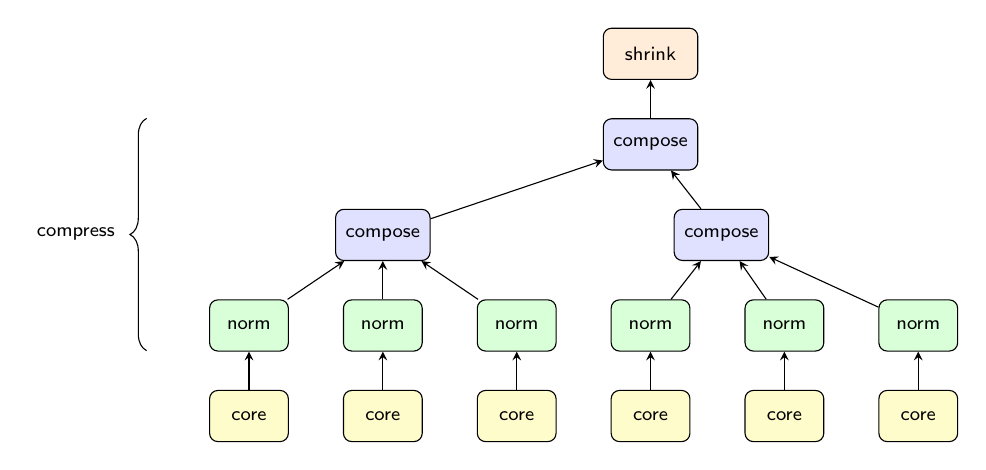
\begin{tikzpicture}[
  box/.style={draw, rounded corners=3pt, minimum height=0.65cm,
              inner sep=3pt, font=\scriptsize\sffamily, align=center},
  core/.style={box, fill=yellow!20, minimum width=1.0cm},
  norm/.style={box, fill=green!15, minimum width=1.0cm},
  comp/.style={box, fill=blue!12, minimum width=1.2cm},
  shrk/.style={box, fill=orange!15, minimum width=1.2cm},
  arr/.style={draw, thin, -stealth},
]
% --- Core shards (row 0) ---
\node[core] (c1) at (0,   0) {core};
\node[core] (c2) at (1.7, 0) {core};
\node[core] (c3) at (3.4, 0) {core};
\node[core] (c4) at (5.1, 0) {core};
\node[core] (c5) at (6.8, 0) {core};
\node[core] (c6) at (8.5, 0) {core};
% --- Normalize (row 1) ---
\node[norm] (n1) at (0,   1.15) {norm};
\node[norm] (n2) at (1.7, 1.15) {norm};
\node[norm] (n3) at (3.4, 1.15) {norm};
\node[norm] (n4) at (5.1, 1.15) {norm};
\node[norm] (n5) at (6.8, 1.15) {norm};
\node[norm] (n6) at (8.5, 1.15) {norm};
\foreach \i in {1,...,6} { \draw[arr] (c\i) -- (n\i); }
% --- Compose layer 1 (row 2) ---
\node[comp] (p1) at (1.7, 2.3) {compose};
\node[comp] (p2) at (6.0, 2.3) {compose};
\draw[arr] (n1) -- (p1);
\draw[arr] (n2) -- (p1);
\draw[arr] (n3) -- (p1);
\draw[arr] (n4) -- (p2);
\draw[arr] (n5) -- (p2);
\draw[arr] (n6) -- (p2);
% --- Compose layer 2 (row 3) ---
\node[comp] (p3) at (5.1, 3.45) {compose};
\draw[arr] (p1) -- (p3);
\draw[arr] (p2) -- (p3);
% --- Shrink (row 4) ---
\node[shrk] (sh) at (5.1, 4.6) {shrink};
\draw[arr] (p3) -- (sh);
% --- "compress" brace on the left (encompasses normalize + compose layers) ---
\draw[decorate, decoration={brace, amplitude=6pt}]
  (-1.3, 0.83) -- (-1.3, 3.78)
  node[midway, left=8pt, font=\scriptsize\sffamily, align=center] {compress};
\end{tikzpicture}
\caption{\label{fig:topo} Recursion topology.
Colors:
\colorbox{yellow!20}{\textsf{\scriptsize core}}\,,
\colorbox{green!15}{\textsf{\scriptsize normalize}}\,,
\colorbox{blue!12}{\textsf{\scriptsize compose}}\,,
\colorbox{orange!15}{\textsf{\scriptsize shrink}}\,.
The tree is illustrative; the actual fan-in and depth depend on the
number of shards.}
\end{figure}

\paragraph{Programs vs.\ verifiers.}
Because of recursive proof aggregation, each recursion step acts as both a
\emph{prover} and a \emph{verifier}: the program executed by the prover
contains the verifier for the previous step's proof system.
For example, the \texttt{compose} program contains the compress
verifier, which verifies \texttt{normalize} and \texttt{compose} proofs.
In the subsections below, when we say ``the \texttt{compose} circuit
verifies a proof,'' we mean that the compose \emph{program}
embeds the compress \emph{verifier} as part of its constraint system.

\paragraph{Verifying key Merkle tree.}
Each recursion circuit type may have multiple \emph{shapes}---distinct
circuit configurations that arise from different chip clusters and
trace dimensions.
A verifying key $\vk$ is derived for each shape, yielding
approximately $181{,}000$ distinct keys in total.
These keys are organized into a Merkle tree whose root
$\mathsf{vk\_root}$ is used to authenticate recursion proofs.

The shapes are enumerated as follows:
\begin{itemize}
\item \textbf{Normalize} (the vast majority of leaves):
one shape per combination of chip cluster, preprocessed and main
stacked BaseFold column counts, and padding column counts.
\item \textbf{Compose}: one shape per arity ($N=1,2,3,4$).
\item \textbf{Shrink}: a single shape.
\end{itemize}

The \texttt{compose} program enforces VK authentication:
it takes Merkle membership proofs for each input proof's verifying key
as part of its witness, verifies them against the Merkle root, and
checks that every input proof's $\mathsf{rpv}.\mathsf{vk\_root}$
equals this root.
The \texttt{normalize} program does not perform VK membership
checks itself; it propagates $\mathsf{vk\_root}$ as a public value,
which the compose verifier then checks for consistency.

Note that, because of the 1-1 normalization, there truly is exactly one \texttt{compose} circuit for each
arity.
If not for the normalization, the number of arity $N$ \texttt{compose} circuits would be $C^N$,
where $C$ is the number of core shard proof shapes.

\subsection{\texttt{core} circuits}\label{sec:core}

To optimize the proof size and prover time,
we introduce core shard circuits that prove
the correctness of RISC-V execution and precompile execution.

The circuits are determined by a ``chip cluster,'' i.e.\ a collection of chips that are proved together
in a single shard.  All inter-shard communication is enabled by passing messages through the global
accumulation bus, which is arithmetized as a \texttt{Global} table present in all shards.

Each chip declares interactions with two possible scopes:
\begin{itemize}
\item \textbf{Local} interactions must balance within the shard.
This is enforced by a LogUp argument (proved via GKR) inside the shard proof.
\item \textbf{Global} interactions need not balance within a single shard.
Instead, each shard computes its net contribution $\sigma\in E(\mathbb{F})$, a point on a
degree-7 elliptic curve over the base field (the ``septic curve''), and outputs it
as a public value.
The contributions are accumulated across all shards during recursion, and the final
completeness check asserts $\sum_i \sigma_i = \mathcal{O}$ (the identity point).
\end{itemize}

Each shard proof attests to the relation
$$
\relation_{\mathrm{shard}}^{(C)} \;=\; \left\{
\left((\mathsf{pv},\sigma);\; \mathsf{trace}\right) \;\Bigg|\;
\begin{array}{c}
\text{All chip constraints in cluster $C$ are satisfied}\\
\text{All local-scope bus interactions balance (via LogUp)}\\
\sigma \text{ is the correct global cumulative sum for the global-scope interactions}\\
\text{Public values $\mathsf{pv}$ are consistent with the trace}
\end{array}
\right\}
$$
where $C$ is the chip cluster determining the circuit, $\mathsf{pv}$ are the shard's public values
(boundary state, digests, etc.), and $\sigma$ is the shard's global cumulative sum.

The clusters are of 4 types:

\begin{enumerate}
\item \textbf{Base core cluster} (\texttt{core}).
Contains all RISC-V instruction chips (ALU, memory load/store, control flow, etc.)
together with infrastructure chips: \texttt{Program} (instruction lookup),
\texttt{ByteLookup} and \texttt{RangeLookup} (preprocessed lookup tables),
\texttt{MemoryLocal} (local memory state),
\texttt{MemoryBump} and \texttt{StateBump} (timestamp management),
\texttt{SyscallCore}, \texttt{SyscallInstrs} (syscall dispatch),
and \texttt{Global} (global bus accumulator).

\item \textbf{Extended core clusters} (\texttt{core+}$P$).
Some precompiles are compact enough to be retained in the core cluster,
avoiding the overhead of a separate shard proof and allowing communication
with their calling context via the local lookup argument.
The retainable extensions are:
\texttt{MemoryGlobalInit}/\texttt{MemoryGlobalFinal},
\texttt{Bls12381Fp}, \texttt{Bn254Fp},
\texttt{Sha256\{Extend,Compress\}} (with their control chips),
\texttt{Uint256Ops}, and \texttt{Poseidon2}.
Extended clusters are generated for subsets of size 0, 1, or all of these extensions,
plus one additional combination (\texttt{core} + memory global + SHA-256 + \texttt{Uint256Ops}).

\item \textbf{Deferred precompile clusters} (\texttt{precompile-}$P$).
Precompiles with high arithmetization costs (in terms of number of columns
in the arithmetization) are proved in their own shards. Each such cluster contains
the precompile-specific chip(s) together with a base set of infrastructure chips:
\texttt{Program}, \texttt{ByteLookup}, \texttt{RangeLookup},
\texttt{SyscallPrecompile}, \texttt{MemoryLocal}, and \texttt{Global}.
They communicate with their RISC-V calling context
via the global lookup argument.
The deferred precompiles include:
elliptic curve operations (Ed25519, Secp256k1, Secp256r1, BN-254, BLS12-381 point add/double),
field arithmetic (BLS12-381 and BN-254 $\mathbb{F}_p$/$\mathbb{F}_{p^2}$ operations),
hash functions (Keccak permutation, SHA-256, Poseidon2),
and big-integer arithmetic (\texttt{Uint256Mul}, \texttt{Uint256Ops}).

\item \textbf{Memory boundary cluster} (\texttt{mem-boundary}).
The global memory argument requires initialization and
finalization: sending the initial memory state into the global bus and receiving the final memory state
from the global bus.
This cluster contains \texttt{MemoryGlobalInit}, \texttt{MemoryGlobalFinal},
\texttt{Global}, and the preprocessed chips.
Note that when memory initialization/finalization is retained into an extended core cluster (type~2),
this standalone cluster is not needed (this happens for very small programs so that the proof can
fit into one shard).
\end{enumerate}





\subsection{\texttt{normalize} circuit}\label{sec:normalize}
The \texttt{normalize} circuit proves the correct verification of a single
core shard proof. Its output is a proof of a fixed shape (\texttt{compress\_shape}),
irrespective of the input shard proof's shape (which varies with the chip cluster).
The circuit takes as witness a shard proof $\pi$, the verifying key $\vk$,
a completeness flag $\mathsf{is\_complete}\in\{0,1\}$,
and a VK Merkle root $\mathsf{vk\_root}$.

The circuit performs two categories of work:
\begin{itemize}
\item \textbf{Shard proof verification.}
A Fiat--Shamir challenger is initialized by observing the verifying key,
and the core shard proof is verified against this challenger
(polynomial commitment openings and constraint satisfaction).

\item \textbf{Aggregation checks.}
Outside the shard verifier, the circuit enforces cross-shard and global correctness:
\begin{itemize}
\item \emph{First-shard PC validation.}
If the shard is the first execution shard,
the circuit asserts that $\mathsf{pc\_start}$ matches the verifying key's start PC.

\item \emph{Global cumulative sum accumulation.}
The output global cumulative sum $\sigma$ is computed by adding
the verifying key's $\mathsf{initial\_global\_cumulative\_sum}$ (if this is the first shard,
otherwise $\mathcal{O}$) to the shard's own $\mathsf{global\_cumulative\_sum}$.

\item \emph{Public values propagation.}
The shard's public values (boundary PCs, timestamps, memory addresses,
digests, exit codes, etc.)\ are propagated into a \texttt{RecursionPublicValues} struct
together with the VK digest and VK Merkle root.
A Poseidon-2 digest of these values is committed as the proof's public output.

\item \emph{Completeness conditions.}
When $\mathsf{is\_complete}=1$, the proof is expected to attest to a
full program execution rather than a single shard, so final boundary
conditions are checked --- including that the program has halted,
the first shard was included,
all ``previous'' boundary values are at their initial state,
and the global cumulative sum equals $\mathcal{O}$
(the identity point on the septic curve).
\end{itemize}
\end{itemize}

Formally, let $\Pi_{\mathrm{shard}}^{(C)}$ be the SNARK for
$\relation_{\mathrm{shard}}^{(C)}$.
Write $\mathsf{pv}$ for the shard's public values
(including its global cumulative sum $\sigma_{\mathrm{shard}}$)
extracted from the proof,
and $\mathsf{rpv}$ for the recursion public values output by the circuit.

$$\relation_{\mathrm{norm}}=\left\lbrace\begin{array}{c|c}
  \mathsf{rpv}
  ;\;
  (\pi,\,\vk,\,C)
  &
  \begin{array}{c}
  \Pi_{\mathrm{shard}}^{(C)}.\mathsf{Verify}(\mathsf{pv},\,\pi)=1\\[4pt]
  \mathsf{rpv}.\mathsf{contains\_first\_shard}=1
    \;\Longrightarrow\;
    \mathsf{pv}.\mathsf{pc\_start}=\vk.\mathsf{pc\_start}\\[4pt]
  \mathsf{rpv}.\sigma \;=\;
    \sigma_{\mathrm{init}} + \mathsf{pv}.\sigma_{\mathrm{shard}},\quad
    \sigma_{\mathrm{init}}:=
    \begin{cases}
      \vk.\sigma_0 & \text{if first shard}\\
      \mathcal{O} & \text{otherwise}
    \end{cases}\\[4pt]
  \mathsf{rpv}\text{ is correctly derived from }\mathsf{pv},\;\vk,
    \text{ and auxiliary inputs}\\[4pt]
  \mathsf{rpv}.\mathsf{is\_complete}=1
    \;\Longrightarrow\;
    \varphi_{\mathrm{complete}}(\mathsf{rpv})
  \end{array}
\end{array}\right\rbrace$$
where $\varphi_{\mathrm{complete}}$ asserts the final boundary conditions
described above (program halted, first shard included, initial boundary
values zero, $\sigma=\mathcal{O}$).

\subsection{\texttt{compose} circuit}\label{sec:compose}

The \texttt{compose} circuit is an $N$-to-1 recursion circuit ($1\leq N\leq 4$)
that consumes $N$ proofs --- each of which may be a \texttt{normalize}
or \texttt{compose} proof --- and produces one proof of
the fixed shape \texttt{compress\_shape}.
Its purpose is to aggregate a batch of proofs that cover
contiguous portions of the execution into a single proof.

The circuit performs two categories of work:
\begin{itemize}
\item \textbf{Proof verification.}
Each input proof $\pi_i$ is verified against its own verifying key $\vk_i$.
The circuit checks that every proof's $\mathsf{vk\_root}$ matches
a single witnessed value, and that each proof's recursion public values
have a valid digest.

\item \textbf{Continuity and aggregation checks.}
The circuit enforces that the $N$ proofs form a contiguous chain:
\begin{itemize}
\item \emph{Sequential continuity.}
For each consecutive pair of proofs,
the ``last'' boundary values of proof~$i$
(PC, timestamp, memory addresses, page indices,
exit code, syscall flags, etc.)
must equal the ``previous'' boundary values of proof~$i{+}1$.
\item \emph{Program identity.}
The $\mathsf{sp1\_vk\_digest}$ and $\mathsf{proof\_nonce}$ are
asserted to be identical across all $N$ proofs.
\item \emph{Accumulation.}
The global cumulative sums $\sigma_i$ from all proofs are summed
(via elliptic curve addition on the septic curve).
The shard counts and $\mathsf{contains\_first\_shard}$ flags
are accumulated.
\item \emph{Completeness conditions.}
When $\mathsf{is\_complete}=1$,
the same final boundary conditions as in the \texttt{normalize} circuit
are checked via $\varphi_{\mathrm{complete}}$.
\end{itemize}
\end{itemize}

Formally, let $\Pi_{\mathrm{comp}}$ denote the SNARK for \texttt{compress\_shape} proofs
(used by \texttt{normalize} and \texttt{compose} alike).
Write $\mathsf{rpv}_i$ for the recursion public values of the $i$-th input proof
($1\leq i\leq N$, $1\leq N\leq 4$),
and $\mathsf{rpv}$ for the aggregated output.

$$\relation_{\mathrm{compose}}=\left\lbrace\begin{array}{c|c}
  \mathsf{rpv}
  ;\;
  (\{\vk_i,\pi_i\}_{i=1}^{N},\;\mathsf{vk\_root})
  &
  \begin{array}{c}
  \forall\, i:\;
    \Pi_{\mathrm{comp}}.\mathsf{Verify}(\mathsf{rpv}_i,\,\pi_i)=1
    \;\wedge\;
    \mathsf{rpv}_i.\mathsf{vk\_root}=\mathsf{vk\_root}\\[4pt]
  \forall\, i<N:\;
    \mathsf{rpv}_i.\mathsf{last\_*}
    = \mathsf{rpv}_{i+1}.\mathsf{prev\_*}\\[4pt]
  \forall\, i:\;
    \mathsf{rpv}_i.\mathsf{sp1\_vk\_digest}
    = \mathsf{rpv}_1.\mathsf{sp1\_vk\_digest}\\[4pt]
  \mathsf{rpv}.\sigma \;=\;
    \textstyle\sum_{i=1}^{N} \mathsf{rpv}_i.\sigma\\[4pt]
  \mathsf{rpv}\text{ boundary values derived from }
    \mathsf{rpv}_1.\mathsf{prev\_*}\text{ and }
    \mathsf{rpv}_N.\mathsf{last\_*}\\[4pt]
  \mathsf{rpv}.\mathsf{is\_complete}=1
    \;\Longrightarrow\;
    \varphi_{\mathrm{complete}}(\mathsf{rpv})
  \end{array}
\end{array}\right\rbrace$$

\noindent
Here ``$\mathsf{last\_*}=\mathsf{prev\_*}$'' is shorthand for the continuity of all
chained boundary values
(PC, timestamp, memory init/finalize addresses, page indices,
exit code, and syscall flags).

\subsection{\texttt{shrink} circuit}\label{sec:shrink}

The \texttt{shrink} circuit is a 1-to-1 recursion circuit that takes the
final complete \texttt{compose} proof and re-proves it with reduced FRI
parameters.
Its purpose is to reduce the proof size: the compress stage uses
FRI parameters sized for a log-trace-area of~$27$, while the shrink
circuit uses parameters for a log-trace-area of~$25$, yielding a
significantly smaller proof that is cheaper to verify in the subsequent
outer proof system (e.g., Groth16).
The shrink circuit has a single fixed shape.

The circuit takes as witness
a compress-stage proof $\pi$,
the verifying key $\vk$ of the input proof,
and a VK Merkle membership proof $\mathsf{mkl}$.

The circuit performs the following work:
\begin{itemize}
\item \textbf{VK Merkle verification.}
The input proof's verifying key is checked against the
VK Merkle tree, ensuring it belongs to the set of
permitted recursion circuits.

\item \textbf{Proof verification.}
The compress-stage proof $\pi$ is verified against its verifying key
$\vk$ using the compress verifier
(the same verifier used inside \texttt{compose}).

\item \textbf{Completeness enforcement.}
The circuit asserts that the input proof is marked
$\mathsf{is\_complete}=1$, meaning it attests to a full program
execution---the program has halted, all shards have been aggregated,
the global cumulative sum equals $\mathcal{O}$, and all boundary
conditions are satisfied.

\item \textbf{Output construction.}
The output recursion public values are derived from the input proof's
public values.
A Poseidon-2 digest of the output public values is committed as the
shrink proof's public output.
\end{itemize}

Formally, let $\Pi_{\mathrm{comp}}$ denote the SNARK for
\texttt{compress\_shape} proofs (as in the \texttt{compose} circuit).
Write $\mathsf{rpv}'$ for the recursion public values extracted from
the input proof and $\mathsf{rpv}$ for the output.

$$\relation_{\mathrm{shrink}}=\left\lbrace\begin{array}{c|c}
  \mathsf{rpv}
  ;\;
  (\vk,\,\pi,\,\mathsf{mkl})
  &
  \begin{array}{l}
  \Pi_{\mathrm{comp}}.\mathsf{Verify}(\mathsf{rpv}',\,\pi)=1\\[3pt]
  \vk \text{ verified against } \mathsf{mkl}\\[3pt]
  \mathsf{rpv}'.\mathsf{is\_complete}=1\\[3pt]
  \varphi_{\mathrm{complete}}(\mathsf{rpv}')\\[3pt]
  \mathsf{rpv}\text{ is correctly derived from }\mathsf{rpv}'
  \end{array}
\end{array}\right\rbrace$$

\noindent
Because shrink enforces completeness, its output serves as the
definitive attestation that the entire program execution is valid.
The shrink proof is then passed to the outer proof system for final
verification.

\section{Proof system instantiations}

In the previous sections, we have described how to arithmetize the correct RISC-V execution of a program
by decomposing it into a collection of tables of field elements, each of which has algebraic constraints
placed on its columns.
Furthermore, we allow tables to ``send'' and ``receive'' messages with multiplicity through a collection of ``interaction kinds''.
All tables are zero padded to have the same height, call it $\mathcal{N}_{row}= 2^{n_{row}}$.
For the RISC-V circuits, we use $n_{row}=22$.
The reason for this padding is that it allows for the verifier to be described as a uniform arithmetic
circuit, independent of the unpadded table heights.
This naturally introduces some prover and verifier overhead; naively, this can be a very large overhead
if one of the tables is wide and short, in which case the padding adds a substantial number of trace cells,
but the Hypercube proof system has a number of mitigations to minimize this overhead.
We will describe some of these mitigations below, especially because one of them is a cryptographic
protocol invented for this particular zkVM context.
First, though, let us describe protocol as if it were actually run on the padded tables:

\begin{enumerate}
\item Treat each column of each table as a multilinear polynomial in $n_{row}$ variables. Use a batch
multilinear polynomial commitment scheme to commit to these polynomials. Let $W$ denote the total
number of columns/multilinear polynomials.
\item Use GKR with $n_{row}$ {\color{red} maybe $\pm 1$} rounds to prove the LogUp argument equating the ``send'' and ``receive'' multisets across
all tables. The output of GKR is a collection of $W$ evaluation claims, one on each column, all at
the same point $\eta$.
\item Use the point $\eta$ as the randomness for the zerocheck sumcheck which proves constraint satisfaction.
Batch the zerocheck sumcheck with the sumchecks which ``prove'' the evaluation claims from LogUp+GKR
(more precisely, the sumchecks
reduce evaluation claims at one point to evaluation claims at another).
The output of this batched sumcheck is again a collection of $W$ evaluation claims, not at a new point
$\eta'$.
\item Use the batch multilinear polynomial commitment scheme to prove these evaluation claims.
\end{enumerate}

If the prover actually materialized the full $W\times \mathcal{N}_{row}$ trace, this would be an
enormous quantity of data.
For example $W\approx 2^{12}$ is in the mid-range of column counts among various ``table clusters'' used
in SP1.
For a 32-bit field such as KoalaBear, this translates into a total of $4\times W\times \mathcal{N}_{row} = 2^{36}$
bytes, or 64 GB.
This is twice the global VRAM of an Nvidia 5090 GPU.
Clearly, keeping around the padding is not feasible.
In order to mitigate these costs, the SP1 proof system uses the following techniques:
\begin{enumerate}
\item Instead of using a batch multilinear PCS directly, we use the jagged polynomial commitment scheme, which
is a sparse PCS designed for exactly the kind of sparsity inherent in the table layout as described above.
This enables the prover and verifier PCS costs to depend only on the size of the unpadded data
(and notably, the verifier PCS costs can be made independent of $W$). For the internal dense PCS,
we use batch BaseFold, which we view as a multilinear PCS for committing to a single multilinear
in \texttt{log\_total\_unpadded\_trace\_area} variables.
The evaluation proof for a point $\eta = \eta_n || \eta_k$ consists of
\item For the sumchecks, the contributions of the padding rows are always easy to compute and don't
scale with the amount of padding. The prover makes frequent use of this fact.
\end{enumerate}

\textbf{Important Note: } The Hypercube proof system verifier can be described as an arithmetic circuit.
The circuit is determined by the total trace area of the unpadded data, and the tables included in the
segment.
Notably, the circuit is \emph{independent} of the individual tables' unpadded heights.
Hence, the total number of verifier circuits can be easily limited to the $\approx 2^{18}$ range,
which makes it feasible to build them all instead of using a VM for recursion.

In the following subsections, we describe each section of the protocol in a bit more detail,
with an eye towards making the soundness analysis in soundcalc more transparent. Whenever a variable
appears in \texttt{typewriter font}, it refers to a parameter in the ``sp1.toml'' file in the soundcalc
repository.

\subsection{LogUp + GKR Details}
{\color{red} TODO: Ask Min about the LogUp+GKR business.}

\subsection{Zerocheck Details}
Recall that we have a trace of height $\mathcal{N}_{row}$ and width $W$ on which we place \texttt{num\_constraints}
algebraic constraints, denoted $C_0, C_1, \ldots, C_{num\_constraints}$.
Each $C_i$ is a polynomial of total degree at most $3$ in $W$ variables, though almost always it depends trivially on most of the variables.
It is useful also to write $W= w_1+ \ldots + w_k$, where $k$ is the number of tables in the cluster,
and to group the constraints by table, so that $C_{i,j}$ refers to the $j$-th constraint on the $i$-th
table.
Let us write $c_i$ for the number of constraints in the $i$-th table, and $p_{i,\ell}$ for the
$\ell$-th column of the $i$-th table.
Finally, let us write $h_i$ for the height of the $i$-th table (not including padding).
The claim for our zerocheck is that, $\forall x\in \{0,1\}^{n_{row}}, \quad i\in [k], \quad j\in [c_i]$:

\begin{equation}
C_{i,j}(p_{i,1}[x], \ldots, p_{i,w_i}[x]) = \left\{ \begin{array}{lr}
0, &x< h_i,\\
C(0,\ldots, 0), & x\geq h_i
\end{array}
\quad \right.
\end{equation}
Note that the constraint evaluation on zero-padding may not result in 0, so at the moment our protocol
does not match exactly with the usual zerocheck.
However, note the following. If $\mathrm{geq}_{h_i}(x)$ is the function which, for $x\in \{0,1\}^{n_{row}}$,
is zero if $x<h_i$ and 1 if $x\geq h_i$, then its multilinear extension $\widehat{\mathrm{geq}}_{h_i}(z)$
is relatively straightforward to evaluate at arbitrary $z\in \mathbb{F}^{n_{row}}$, using the following
recursion relation. Write $z = (z_0, z_{rest})\in \mathbb{F}\times \mathbb{F}^{n_{row}-1}$, and write $h_i = h_{i,0} * 2^{n_{row}-1} + h_{i, rest}$.
Then, we have:
\[
\widehat{\mathrm{geq}}_{h_i}(z) = z_0\cdot(1-h_{i,0}) + \widehat{\mathrm{eq}}(z_0, h_{i,0})\cdot \widehat{\mathrm{geq}}_{h_{i,rest}}(z_{rest})
\]


To prove this, first, we sample a random $\zeta \in \mathbb{F}^{n_{row}}$, $\lambda\in \mathbb{F}, \alpha \in \mathbb{F}$,
and turn this collection of claims into the single sumcheck claim:

\begin{equation}
\sum_{i=0}^{k-1}\sum_{j=0}^{c_i-1} \lambda^i\alpha^j \widehat{\mathrm{geq}}_{h_i}(\zeta)=\sum_{x\in \{0,1\}^{n_{row}}} \widehat{\mathrm{eq}}_\zeta(x)\sum_{i=0}^{k-1} \lambda^i\sum_{j=0}^{c_i-1} \alpha^j C_{i,j}(p_{i,1}[x], \ldots, p_{i,w_i}[x])
\end{equation}


\end{document}
